\section{Musique}

\subsection{Partition}

Une partition est un document contenant toutes les informations jugées nécessaires par l'auteur pour pouvoir interpréter une musique. Elle est composée de portées qui contiennent elles-même des mesures. Une mesure dispose d'une clé, d'une armure et d'une signature si elle est la première de sa portée et une ensemble de notes, accords ou silences.

%image d'une partition

\subsection{Durée}

La durée est le temps pendant laquelle la note est jouée. La durée n'est pas exprimée sous forme de valeur fixe mais comme une proportion relative à la mesure. En effet, la durée de la mesure dépend de sa signature et du tempo (expliqués plus tard). 


\subsection{Signature}

La signature symbolise le référentiel de la durée de la mesure. Elle peut être représentée sous forme d'une fraction. Le numérateur permet de définir la durée totale de la mesure et le dénominateur la durée d'un temps dans la mesure. 

\subsection{Note}

Une note est définie par sa hauteur et sa durée. La hauteur caractérise la fréquence du son d'une note. Cette fréquence est divisée en 8 intervalles appelé octave. Cette octave est divisée en 7 hauteurs : do, ré, mi, fa, sol, la et si. En ce qui concerne la durée de la note, elle est indiquée par la tête de la note et la présence ou non de croches. Si l'on ne prend pas en compte les croches, il existe 4 types de durées pour une note : carrée, ronde, blanche et noire. Une note carrée vaut 2 rondes, 4 blanches et 8 noires. Afin d'exprimer une durée plus courte que celle de la noire, on peut lui rajouter un ou plusieurs symboles de croches. La durée de la note s'en retrouve divisée par deux.

\par
Dans notre programme tout comme dans MusicXML, nous utilisons la notation anglo-saxonne. Elle diffère de la notation française par la façon dont est exprimée la hauteur et la durée de la note. Do, ré, mi, fa, sol, la et si sont remplacés respectivement par A, B, C, D, E, F et G. Concernant la durée, ce sont simplement des fractions. Par exemple, la blanche est un 1/2 (half) et la noire 1/4 (quarter).

%image wiki note


\subsection{Tempo}

Le tempo contient un type (une noire par exemple) et un nombre par minute. Ainsi, le tempo \emph{60 à la noire} signifie qu'il y a, dans une minute, 60 noires ou bien 30 blanches. Un élément musical possède aussi une liste de symboles musicaux. Un symbole musical représente une notation qui peut être une nuance comme un point ou encore un répétition par exemple.


\subsection{Symboles musicaux}

Nous désignons par symbole musical, chaque artefact influençant la manière de jouer une note ou un groupe de notes.


Symboles unaires : 

 \begin{music}
 
 \instrumentnumber{1} % nombre de voix
 \generalmeter{\meterfrac{4}{4}} % mesure 4/4
 %\setname 1{chant} %nom de la portée
 
\startextract
\metron{\qu}{60} % tempo
\def\atnextbar{\znotes\loffset{0.7}{\centerbar{\Fermataup l\wh j}}\en}% point d'orgue
\bar
\NOTes\trrml j\ha j \en % tremolo double

%accent
\Notes\ibu0f3\busfz0\qb0f\bupz0\qb0g\bust0\qb0h\buppz0\qb0i\busf0\qb0j\butext0\tqh0k\en
\Notes\Ibl0lg5\blsfz0\qb0l\blpz0\qb0k\blst0\qb0j\blppz0\qb0i\blsf0\qb0h\bltext0\tqb0g\en

\endextract
 
 \end{music}
 
 Symboles binaires : 
 
  \begin{music}
 
 \instrumentnumber{1} % nombre de voix
 \generalmeter{\meterfrac{4}{4}} % mesure 4/4
 %\setname 1{chant} %nom de la portée
 
\startextract
\notesp\triolet n\isluru0l\Ibl0ln2\qb0{lm}\tslur0n\tqb0n\en % triolet
\endextract
 
 \end{music}
 
 
 Symboles de répétitions : 
 
  \begin{music}
 
 \input musixps
 \instrumentnumber{1} % nombre de voix
 
\startextract
\NOTes\ha g\en
\leftrepeat
\NOTes\ha h\en
\leftrightrepeat
\NOTes\ha i\en
\rightrepeat
\NOTEs\wh j\en

\endextract
 
 \end{music}
 
 
 Plusieurs portées et voix :
  
 \begin{music}
 
 \instrumentnumber{2} % 2 instruments
 
 \setstaffs 1{2} % instrument 1 (en bas) : 2 portées
 
 \setclef{1}{60} % clef de fa (6) en 1, clef de sol (0) en 2
 \generalmeter{\meterfrac{4}{4}} % mesure 4/4
 \setname 1{piano} %
 \setname 2{chant} %
 \parindent 10mm % pour éviter la collision de piano avec l'accolade
 \startextract
 % {{bleu|1re mesure}}
 \Notes 
 \ha J | % chgt portée, même instr
 \zhu{c e}\hu g & % chgt instr ; pas d'espace entre } et \hu
 \islurd0c\ibu0d0\qb0{c c c}\tslur0d\tbu0\qb0d 
 \enotes % assure l'alignement
 %
 \Notes 
 \ha N | % chgt portée, même instr
 \zhu{g i}\hu k & % chgt instr
 \qa{e d} 
 \enotes 
 \bar % après toutes les notes de la mesure, pour toutes les voix
 % {{bleu|2e mesure}}
 \Notes
 \qa J | 
 \zqu{c e}\qu g &
 \islurd0c\ibu0d0\qb0{c e} 
 \enotes
 %
 \Notes
 \qa N |
 \zqu{g i}\qu k &
 \qb0{d}\tslur0d\tbu0\qb0d
 \enotes
 %
 \Notes
 \ha J | 
 \zhu{c e}\hu g &
 \ha c 
 \enotes
 %
 \endextract
 
 \end{music}


\subsection{Arbre rythmique}

\par
Dans notre application, les durées des éléments constituant les mesures sont représentées sous forme d'arbres rythmiques. Comme décrit dans l'article \cite{agon}, \enquote{un arbre rythmique est défini comme un couple (D S) où D est une fraction (< 0) et S est une liste de n-éléments définissant n-proportions de D. Chaque élément de S peut-être soit un entier, soit un arbre rythmique.}

\par
Les images suivantes sont des exemples d'arbres rythmiques, en haut, et la partition correspondante, en bas.


\begin{minipage}[c]{.46\linewidth}
  \centering
  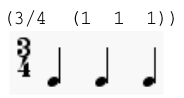
\includegraphics[width=0.5\textwidth]{rt1.png}\\[1cm]
\end{minipage}
\hfill
\begin{minipage}[c]{.46\linewidth}
  \centering
  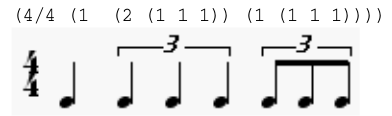
\includegraphics[width=0.9\textwidth]{rt2.png}\\[1cm]
\end{minipage}

%silence et liaison



